\section{Architettura}
L'architettura del progetto è basato sul pattern Model-View-Controller (MVC), seguendo le linee guida del framework Laravel per la creazione della web application.


\subsection{Diagrammi delle classi}

Il diagramma delle classi è diviso principalmente in due sezioni:
\begin{itemize}
    \item Generazione Captcha;
    \item Download e elaborazione delle immagini.
\end{itemize}

\subsubsection{Generazione del Captcha}

\begin{landscape}
\begin{figure}[H]
    \centering
    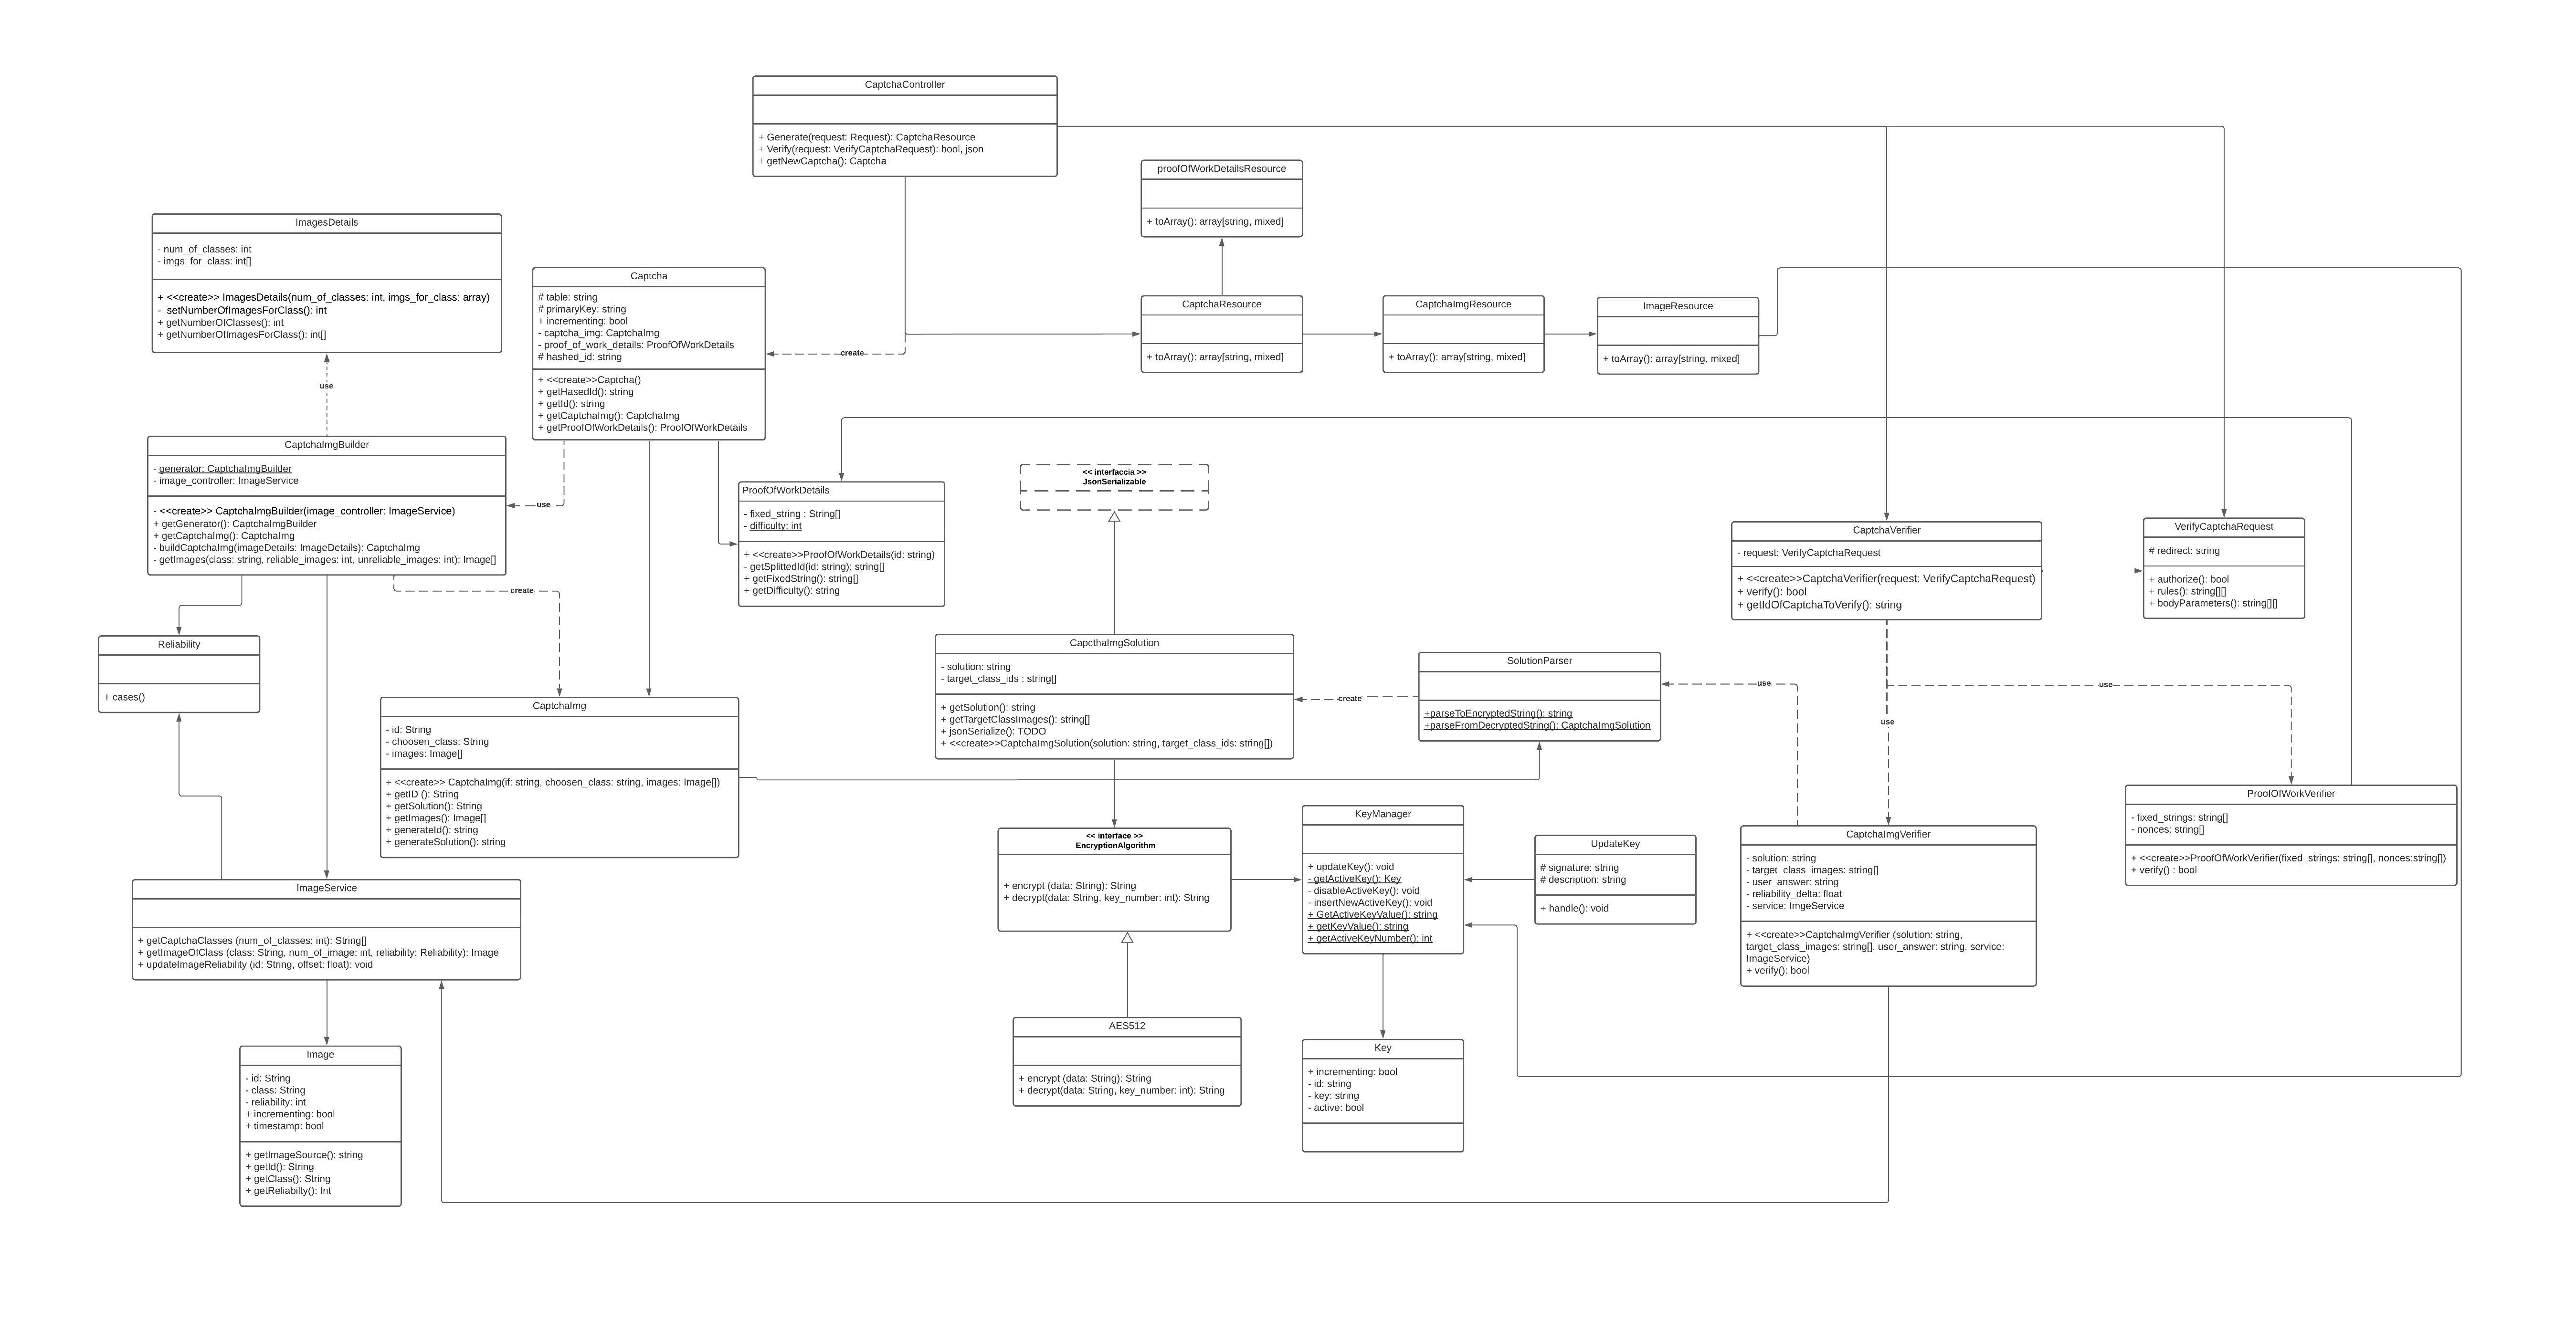
\includegraphics[scale = 0.6]{img/generale.png}\\
    \caption{Diagramma delle classi. Generazione del Captcha}
\end{figure}
\end{landscape}
\newpage

La figura sopra riportata rappresenta il back-end dell'applicazione, ha il compito di
\begin{itemize}
    \item Costruire il Captcha combinando:
    \begin{itemize}
        \item Le immagini;
        \item L'honeypot;
        \item Il proof of work.
    \end{itemize}
    \item Verificare le risposte date dall'utente;
    \item Gestione delle chiavi e criptazione.
\end{itemize}

In particolare:
\begin{itemize}
    \item \textbf{CaptchaController}: componente principale, raggruppa le funzionalità principali (di creazione e di verifica) in un unica classe;
    \item \textbf{Captcha}: componente di generazione del captcha, esso combina le immagini e il proof of work e lo ritorna alla pagina richiedente;
    \item \textbf{CaptchaImgBuilder}: componente di creazione effettivo del captcha parte delle immagini;
    \item \textbf{ProofOfWorkDetails}: componente di generazione dei dati neccessari per il proof of work;
    \item \textbf{CaptchaVerifier}: componente di verifica, richiama le classi di verifica del captcha immagini e del proof of work e ritorna. In base ai controlli determina il superamento o meno del captcha;
    \item \textbf{CaptchaImgVerifier}: componenete di verifica del captcha immagini;
    \item \textbf{ProofOfWorkVerifier}: componente di verifica del proof of work;
    \item \textbf{EncryptionAlgorithm}: interfaccia di criptazione e decripazione;
    \item \textbf{KeyManager}: componenete di gestione delle chiavi di criptazione.
\end{itemize}

DESCRIZIONE DEL PROCESSO

\subsubsection{Download e elaborazione delle immagini}

\begin{figure}[H]
    \centering
    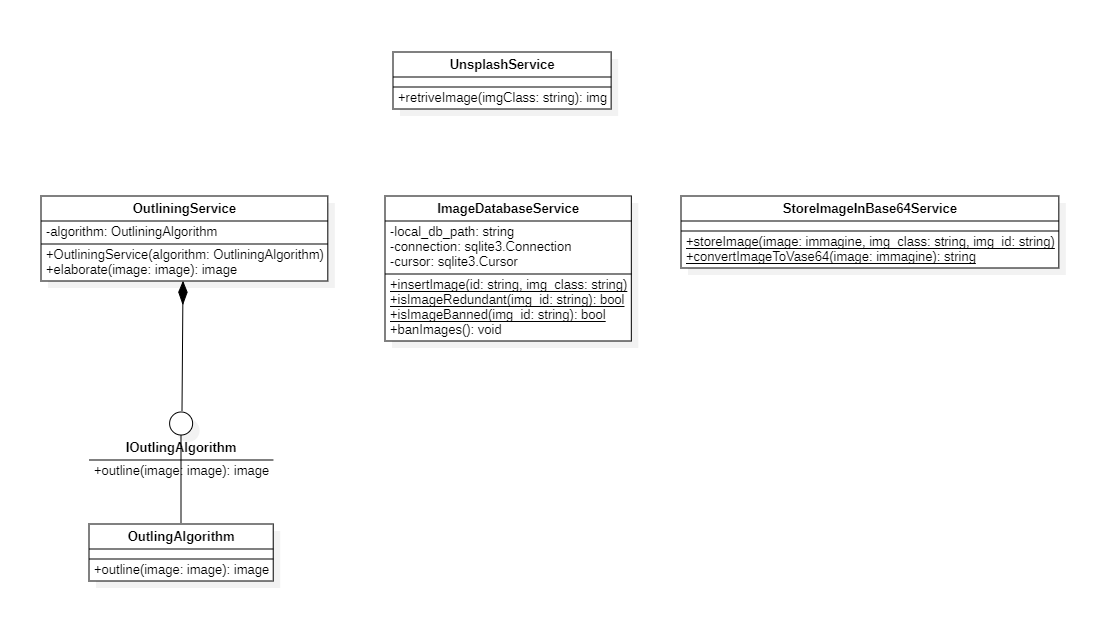
\includegraphics[scale = 1.0]{img/downloadImg.png}\\
    \caption{Diagramma delle classi. Recupero delle immagini da Unsplash}
\end{figure}

La figura sopra riportata rappresenta il metodo di download delle immagini dal sito di Unsplash, la rielaborazione di tali immagini e
il metodo di salvataggio. Vengono eseguiti con il seguente ordine:
\begin{enumerate}
    \item Viene scaricato l'immagine di una determina classe;
    \item Rielaborazione dell'immagine eliminando i colori e tenendo solo il contorno.
    \item Conversione dell'immagine in base64;
    \item Salvataggio dell'immagine del database.
\end{enumerate}

In particolare:
\begin{itemize}
    \item \textbf{UnsplashService}: download dell'immagine;
    \item \textbf{OutliningService}: elaborazione dell'immagine;
    \item \textbf{OutilningAlgorithm}: algoritmo di elaborazione dell'immagine;
    \item \textbf{StoreImageInBase64Service}: conversione dell'immagine in base64;
    \item \textbf{ImageDatabaseService}: salvataggio dell'immagine.
\end{itemize}

\subsection{Architettura di dettaglio}

\subsubsection{Strategy pattern}

\begin{figure}[H]
    \centering
    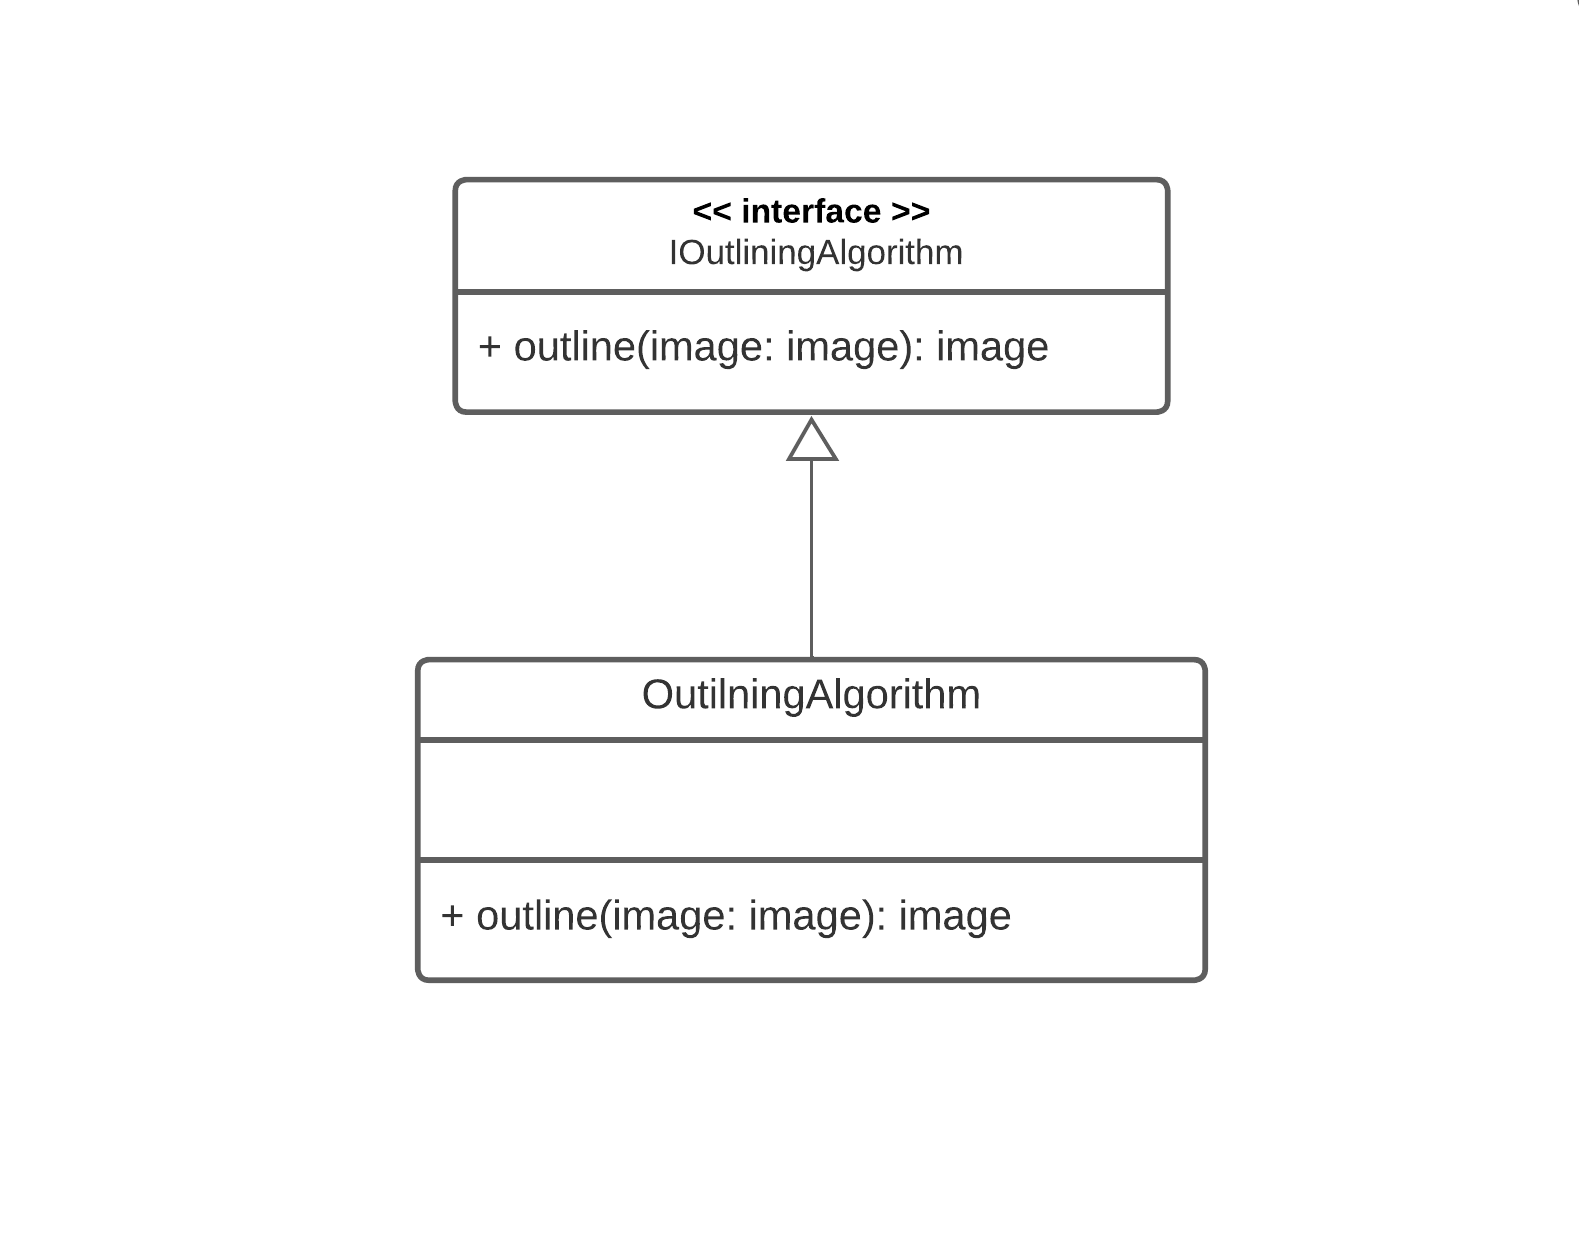
\includegraphics[scale = 1.0]{img/outlineStrategy.png}\\
    \caption{Strategy pattern dell'algoritmo di rielaborazione dell'immagine}
\end{figure}

Attualmente, la classe astratta "IOutliningAlgorithm" ha una sola classe concreta che rappresenta l'unico algoritmo 
di scontornaggio implementato. Tuttavia, è progettata in modo da consentire l'estensione per l'implementazione di ulteriori 
algoritmi di scontornaggio in futuro. Ciò significa che se si desidera aggiungere nuovi algoritmi di scontornaggio, 
sarà possibile creare nuove classi che estendono l'interfaccia astratta "IOutliningAlgorithm". 
Questa flessibilità consente di espandere il sistema per includere più algoritmi di scontornaggio senza dover 
modificare la struttura di base.

\begin{figure}[H]
    \centering
    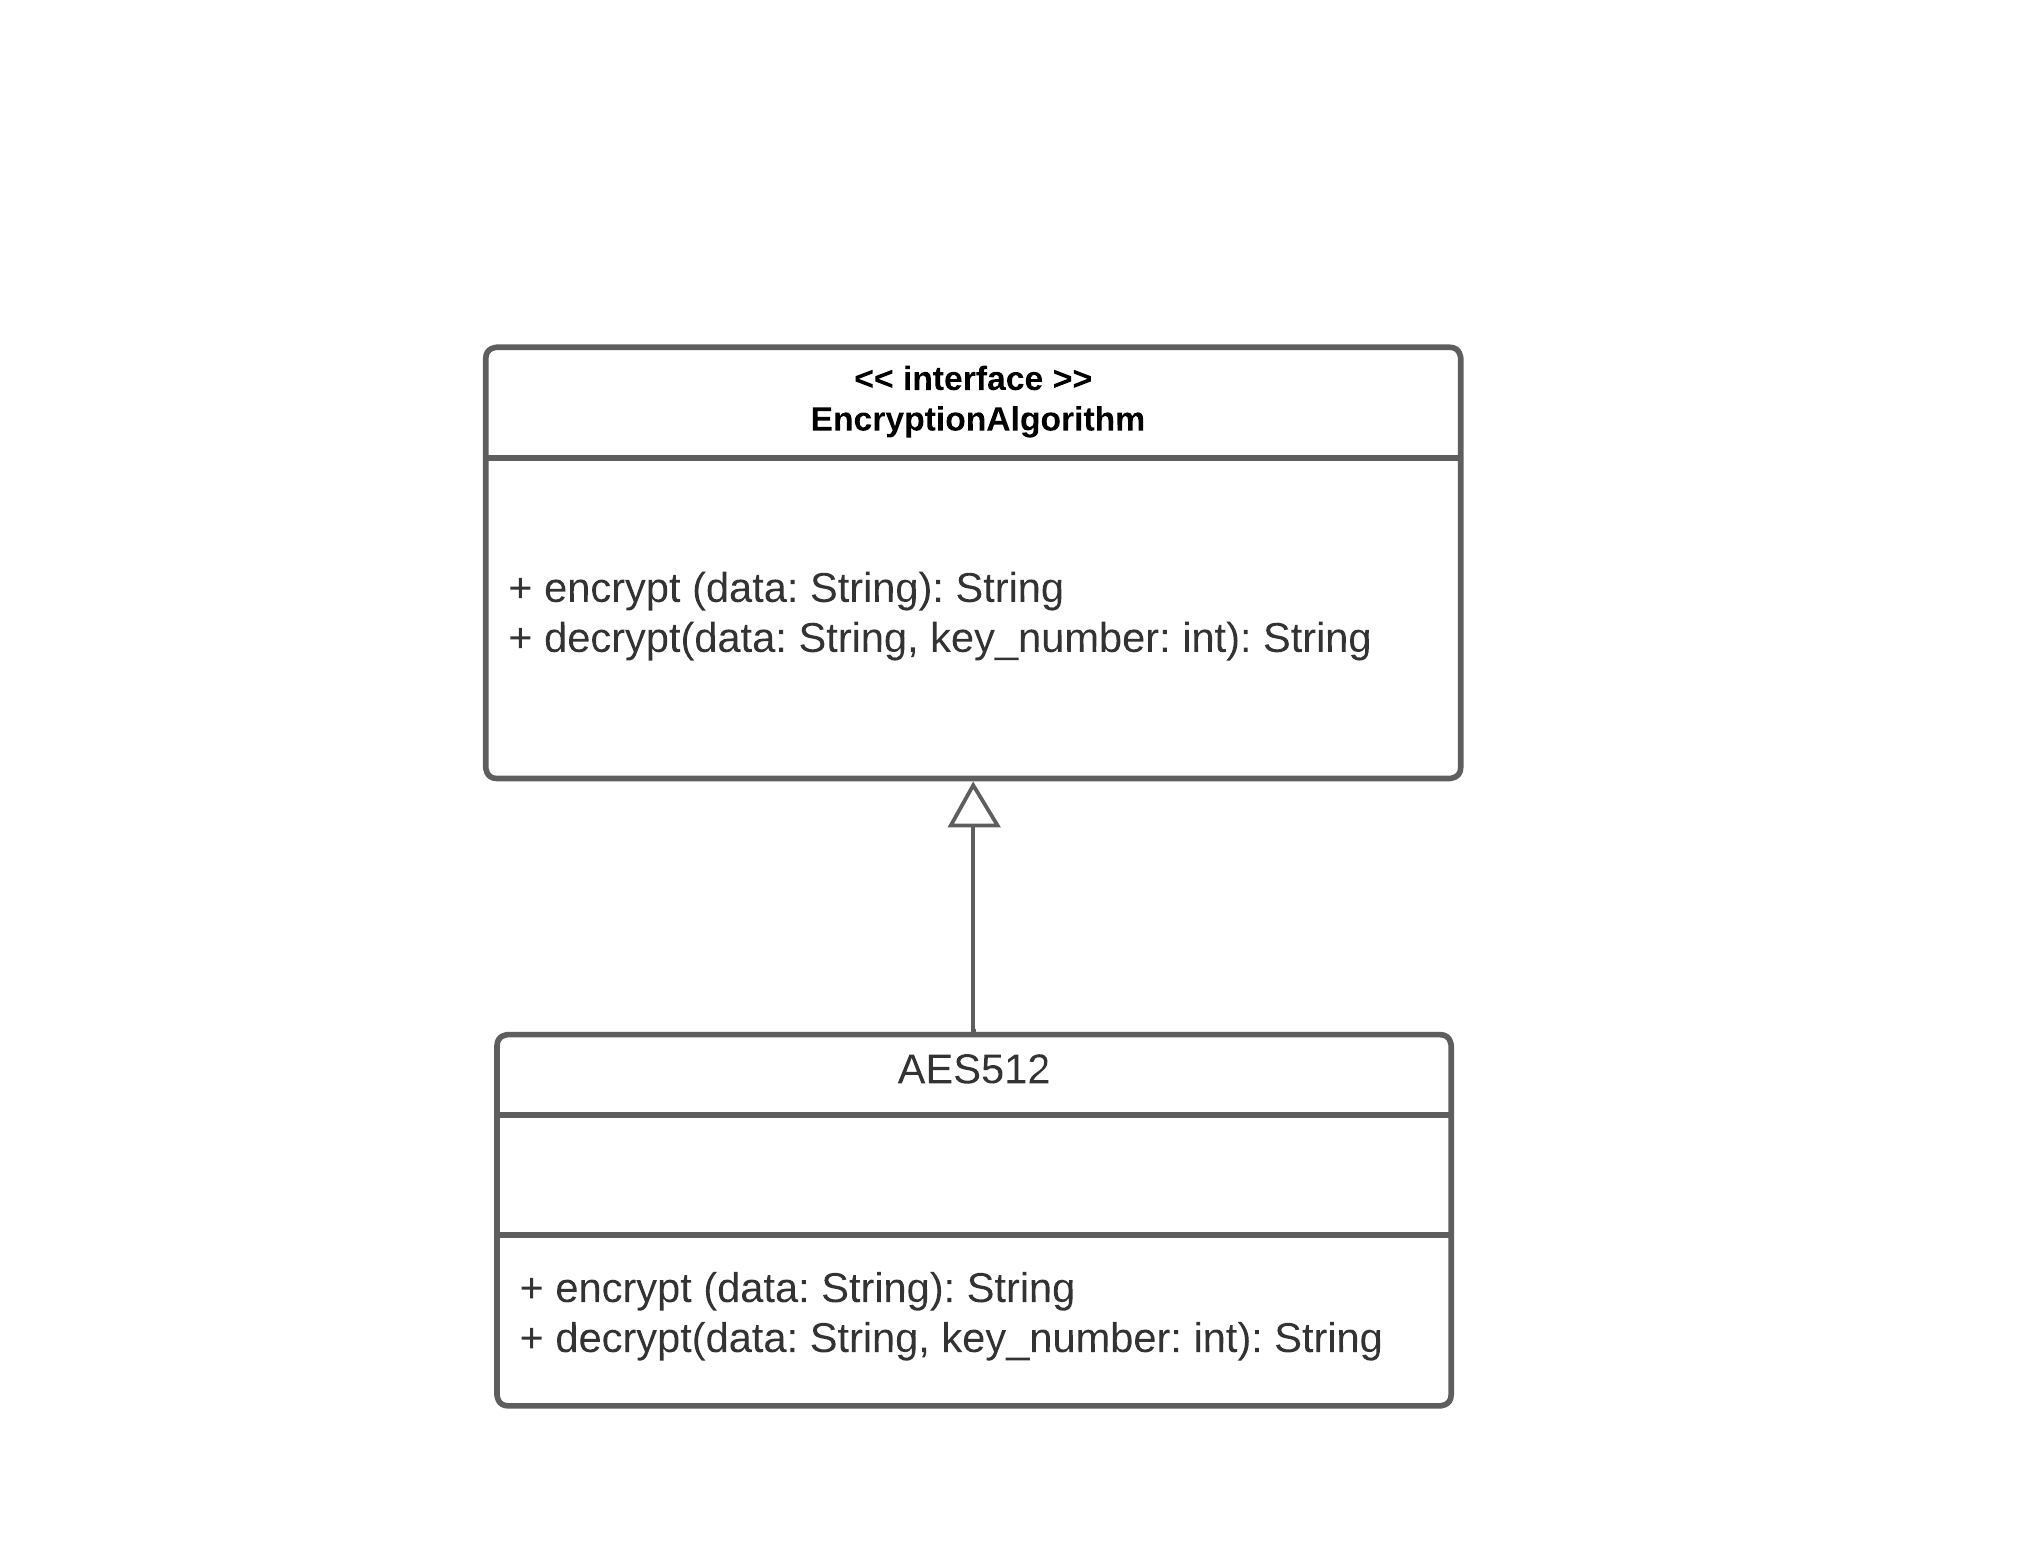
\includegraphics[scale = 1.0]{img/criptStrategy.png}\\
    \caption{Strategy patter dell'algoritmo di criptaggio}
\end{figure}

Anche qua la classe astratta "EncryptionAlgorithm" ha una sola classe conreta per il motivo sopra citata.

\subsubsection{Singleton}

\begin{figure}[H]
    \centering
    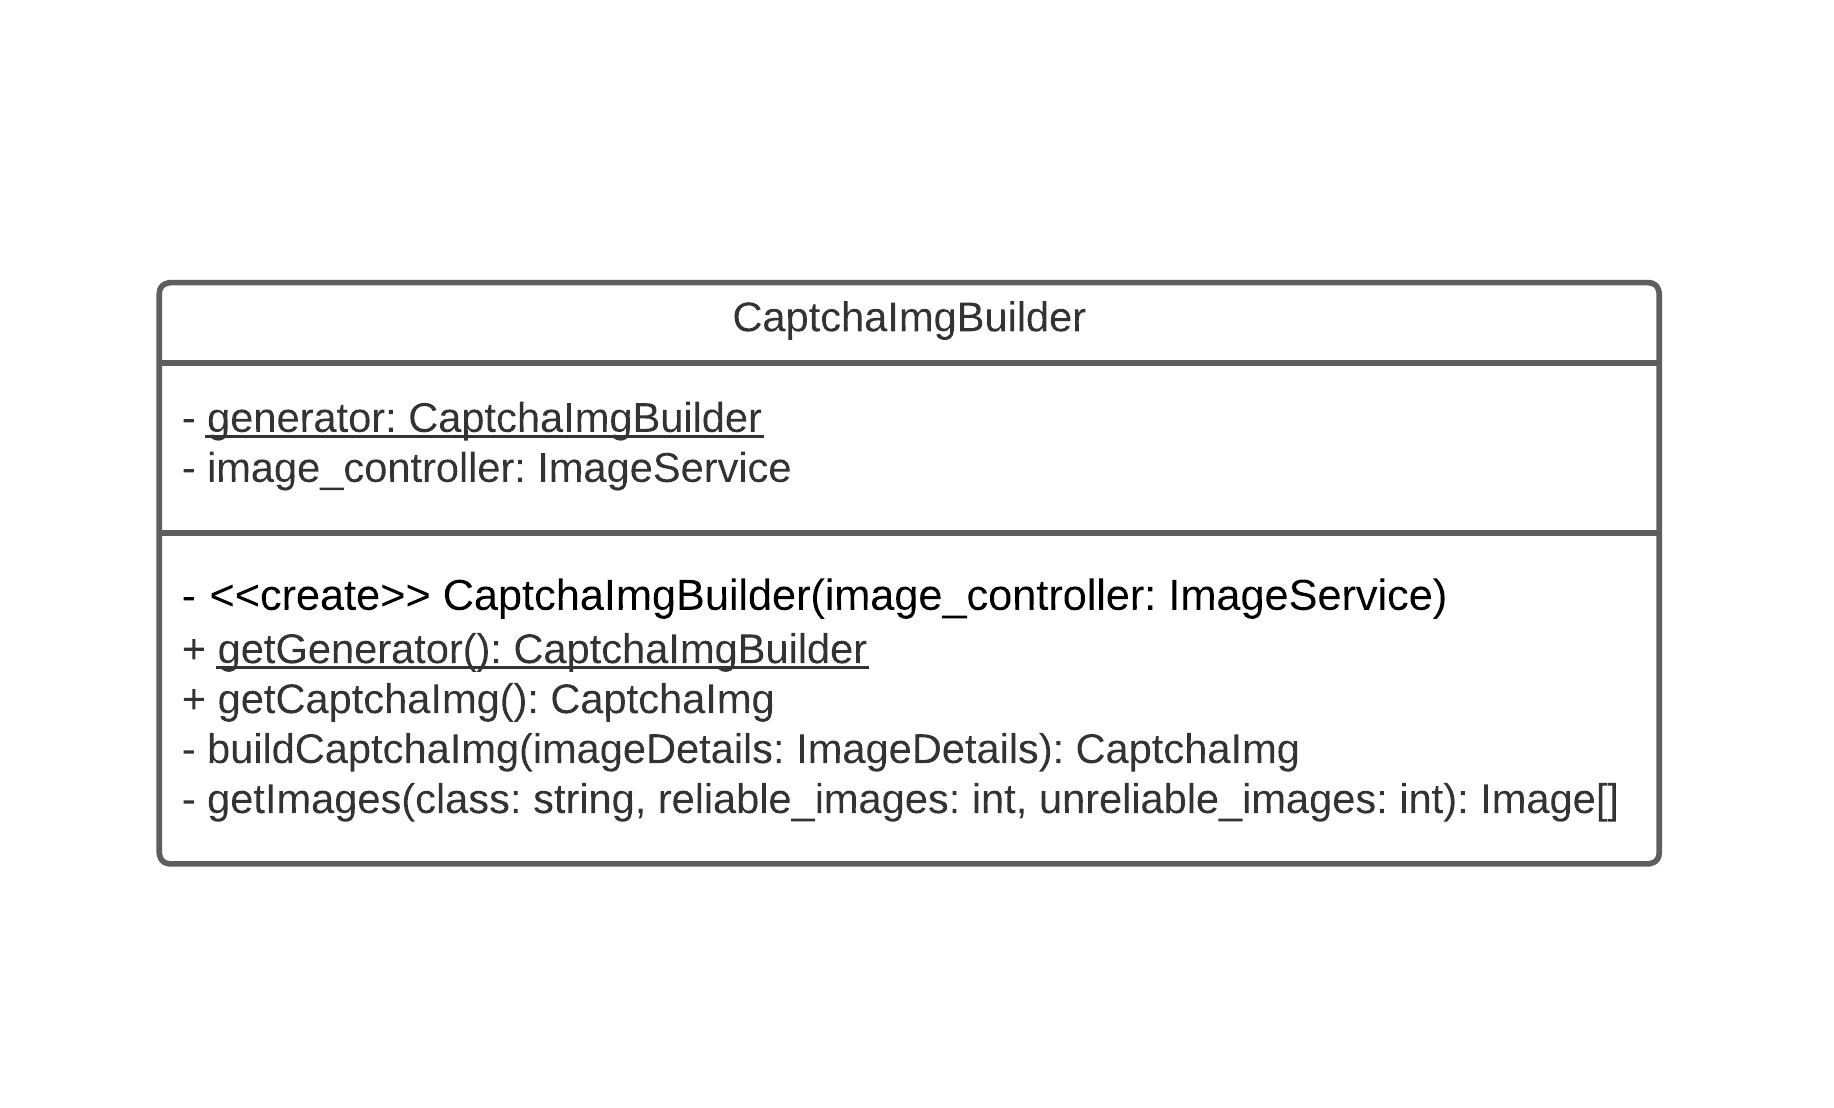
\includegraphics[scale = 1.0]{img/singleton.png}\\
    \caption{Singleton pattern}
\end{figure}